\title{Generalizing n-Dimensional Grid Maps Handling and Neighbor Cells Extraction}
\author{
        Javier V. G\'omez \\
        RoboticsLab\\
        Carlos III University of Madrid\\
        E-mail: jvgomez@ing.uc3m.es\\
        Website: www.javiervgomez.com\\
        Document: V 1.1
}
\date{\today}

\documentclass[12pt]{article}

\usepackage{hyperref}
\usepackage{amssymb}
\usepackage{amsmath}
\usepackage{enumerate}
\usepackage{graphicx}
\usepackage{listings}
\DeclareGraphicsExtensions{.pdf}
\graphicspath{{images/}}

\usepackage{color}

\definecolor{dkgreen}{rgb}{0,0.6,0}
\definecolor{gray}{rgb}{0.5,0.5,0.5}
\definecolor{mauve}{rgb}{0.58,0,0.82}

\lstset{frame=tb,
  language=c++,
  aboveskip=3mm,
  belowskip=3mm,
  showstringspaces=false,
  columns=flexible,
  basicstyle={\footnotesize\ttfamily},
  numbers=none,
  numberstyle=\tiny\color{gray},
  keywordstyle=\color{blue},
  commentstyle=\color{dkgreen},
  stringstyle=\color{mauve},
  breaklines=true,
  breakatwhitespace=true
  tabsize=3
}

\begin{document}
\maketitle

\begin{abstract}
\noindent Grid maps are extensively used in many different algorithms. Among the different grid map types we are focusing on rectangular (or cubic)
grid map with \emph{a priori} unknown number of dimensions. We are detailing the main problems that arise when working with this
type of data structure: extraction and validation of 4-connectivity neighbors for a given cell, conversion from index to coordinates (and vice-versa)
and the mathematical generalization to n-dimensional grids. Also, we are detailing a generic implementation available as free software.
\end{abstract}

\section{Introduction}
Mathematically, grid maps are data structures that divide (discretize) the space in cubes (hypercubes) of n dimensions. They are commonly
used in artificial intelligence algorithms, such path planning. Although their mathematical definition is clear and simple, it is not
that easy to work with them from a practical point of view. Therefore, in this report we are detailing the mathematical generalization
of common operations with cubic grid maps and how to implement them. Another useful tutorial on grid maps (but only for 2D) can be found 
in \url{http://www-cs-students.stanford.edu/~amitp/game-programming/grids/} which includes triangular and hexagonal grids.


The main reason of this report is that, when trying to implement such structures, it becomes difficult to generalize. For example,
boost::multi\_array library provides tools to create n-dimensional arrays in which the number of dimensions has to be known in
compilation time, which is an important limitation. We detected a lack in the available software of n-dimensional grid maps in which
the size can be dynamic, even in the number of dimensions, in run time. Therefore, we came up with the formulation described in this document
in which all the operations are parametrized by the number of dimensions and their size. This is probably not a novel work, but we were not
able to find any similar document.

For any comment or questions about the formulation, implementation, this document or whatever, please, do not hesitate to contact the author.

\paragraph{Note}
A strong mathematical background is NOT required to understand this document, not even a strong programming background. The formulation
and implementation detailed in the following lines have been tested in complex algorithms.

\section{Definitions}
For simplicity, we are assuming cubic (or hyper-cubic) grids. This mean that the cell size is the same in all dimensions. However, the
same applies for any parallelogram-based grid map. Hence, we define an n-dimensional grid map as the set of cells correctly ordered whose
dimensions are consistent in terms of size. In other words, if the first row has 5 columns, the second row will also have 5 columns.


An n-dimensional grid map $G$ is composed by $n_{dims}$ dimensions. The size of each dimension is stored in a vector 
$d = [d_0, d_1,\dots,d_{n-1}]$ and the size of the total grid map is 
$$size(G) = \prod_{i=0}^{n-1}d_i = d_0\cdot d_1\cdot\dots\cdot d_{n-1}$$

\noindent Each cell within the grid map can be accessed in a double manner:
\begin{enumerate}
 \item By its \textbf{index}. Each cell has a specific index within the grid map which completely depends on the ordering convention chosen.
 \item By its \textbf{coordinates}, giving a set of coordinates $c = [c_0, c_1,\dots,c_{n-1}]$.
\end{enumerate}
The conversion from index to coordinates and vice-versa is trivial but can be very painful if one does not have a good day. Therefore,
it is detailed in section~\ref{sec:helper}


In figure~\ref{fig:grid_example} examples of 2D and 3D grid maps are shown. Note that the index ordering is not unique. In this case we
have chosen this ordering since it is easier to match with the physical dimensions of the grid (dimension 0 is x, dimension 1 is y, and so on). 
For instance, in computer vision it is almost an standard to place the first cell (pixel) in the top-left of the grid map (image) with the
dimension 0 (rows) going downwards and dimension 1 (columns) leftwards. In any case, the formulation should valid in any case. However,
we recommend to review it as minor adjustments could be required.

\begin{figure}[ht]
    \centering
    \includegraphics[width=\textwidth]{grid_definitions}
    \caption{Example of a 2D and a 3D grid map. Usually, 3D grid maps are represented with cubes. The numbers within the cells are
    the indices of those cells.}
    \label{fig:grid_example}
\end{figure}


\section{General Neighbor Extraction}
In this section we detail the generalization of the neighbor extraction in a \textbf{4-connectivity} scheme. In order words,
only cells which are \emph{touching} other cells (sharing faces) are considered neighbors. In case you are interested in a 8-connectivity
formulation and you want it to be included in this document, please let the authors know.

In order to help the reader, we will detail the general formulation by explaining the 2D case, expanding it to 3D and later generalizing 
to n-dimensions. Along the document, we are working with the cells indices. When the dimensions of the grid are known it is easy
to build a vector of size $n_{dims}$ and check the neighbors by doing $\pm1$ in each coordinate. However, in our case the dimensions
of the grid are not known until execution. Therefore, to generalize it is much easier and efficient to work indices, as we are showing
in the next paragraphs.

\subsection{2-dimensional Neighbor Extraction}
In a 2-dimensional map, the neighbor extraction is almost direct. In this case, there are 4 neighbors, as shown in figure~\ref{fig:2d_neighbors}.

\begin{figure}[ht]
    \centering
    \includegraphics[width=0.5\textwidth]{2d_neighbors}
    \caption{4 neighbors highlighted in red of cell with index 7 (shaded) in a 2D grid map.}
    \label{fig:2d_neighbors}
\end{figure}

Now let us focus on the case shown in figure~\ref{fig:2d_grid}: a general 2D grid map where $d=[d_0,d_1]$ is not known in advance. The neighbors of a cell with index $i$,$N(i)$ are given by the following expression:

\begin{equation}
  \mathcal{N}(i) =
  \begin{cases}
      \begin{cases}
      i-1\\
      i+1\\
    \end{cases} & \text{for dimension 0}\\
     \begin{cases}
      i-d_0\\
      i+d_0\\
    \end{cases} & \text{for dimension 1}\\
  \end{cases}
  \label{eq:2d_neighbors}
\end{equation}


\begin{figure}[ht]
    \centering
    \includegraphics[width=0.6\textwidth]{2d_grid}
    \caption{4 neighbors highlighted in red of cell with index $i$ (shaded) in a generic 2D grid map.}
    \label{fig:2d_grid}
\end{figure}

In the case shown in figure~\ref{fig:2d_grid}, we have $ i = 2d_0+2$. Hence, its neighbors will be:

\begin{equation}
  \mathcal{N}(i) = \mathcal{N}(2d_0+2) =
  \begin{cases}
      \begin{cases}
      i-1 = 2d_0+3\\
      i+1 = 2d_0+1\\
    \end{cases} & \text{for dimension 0}\\
     \begin{cases}
      i-d_0 = d_0+2\\
      i+d_0 = 3d_0+2\\
    \end{cases} & \text{for dimension 1}\\
  \end{cases}
\end{equation}

\subsubsection{Checking neighbors validity}
If the queried index $i$ is in one of the borders of the grid map, it will happen that the neighbors are not valid. Recalling 
figure~\ref{fig:2d_neighbors}, imagine that we want to extract the neighbors of $i=19$. According equation~(\ref{eq:2d_neighbors}),
the set of neighbors would be $\mathcal{N}(19)={18,20,14,24}$. However, we can see that the cells with index 20 does not exist. The returned neighbor is out of bounds of the given grid map. Also, $\mathcal{N}(14)={13,15,9,19}$ gives index 15 as neighbor. In this case it is supposed to be a neighbor in dimension 0, but its value for dimension 1 (coordinate 1) is $c_1=3$ while this value for cell index 14 is $c_1=2$. Therefore, it is not a neighbor.

This checking is easy if we were working with coordinates. Coordinates of cell index 14 are $c(14)=[4,2]$. Neighbors in each dimension can be obtained by doing $\pm1$ in each dimension. This means $\mathcal{N}([4,2])={[3,2],[5,2],[4,1],[4,3]}$, where $[5,2]$ is out of bounds of the grid. As we decided to work with cell indices, the following has to be checked:

\begin{itemize}
 \item \textbf{Dimension 0:} Are the 2 neighbors in the same row ($c_1$) that the queried cell?
 \item \textbf{Dimension 1:} Are the 2 neighbors within grid bounds?
\end{itemize}

The mathematical expression to check if the given indices are neighbors of $i$ are as follows:

\begin{enumerate}
 \item Neighbors of $i$ in dimension 0 are valid if (operator $[\cdot]$ means the integer part, this is, the integer number immediately below):
  \begin{equation}
   \left[(i\pm1)/d_0\right] = \left[i/d_0\right]
  \end{equation}

 \item Neighbors of $i$ in dimension 1 are valid if:
 
   \begin{equation}
      \begin{array}{lcc}
	i-d_0 \geq 0 \\
	i+d_0 < size(g) = d_0\cdot d_1
      \end{array}
      \end{equation}
\end{enumerate}


\subsection{3-dimensional Neighbor Extraction}
Following the same procedure as for 2D grid maps, the neighbors extraction in a 3D grid map whose dimensions are not known until run time, as shown in figure~\ref{fig:3d_grid}, is detailed in the following lines. In this case, there are a maximum of 6 neighbors. The drawing of a 3D grid map with undefined dimensions size is omitted since it is hard to understand. The following expression is valid to get the neighbors of such grid map:

\begin{equation}
  \mathcal{N}(i) =
  \begin{cases}
      \begin{cases}
      i-1\\
      i+1\\
    \end{cases} & \text{for dimension 0}\\
     \begin{cases}
      i-d_0\\
      i+d_0\\
    \end{cases} & \text{for dimension 1}\\
     \begin{cases}
      i-d_0\cdot d_1\\
      i+d_0\cdot d_1\\
    \end{cases} & \text{for dimension 2}\\
  \end{cases}
  \label{eq:3d_neighbors}
\end{equation}

\begin{figure}[ht]
    \centering
    \includegraphics[width=0.6\textwidth]{3d_grid}
    \caption{6 neighbors highlighted in red of cell with index $i$ (shaded) in a 3D grid map.}
    \label{fig:3d_grid}
\end{figure}

\subsubsection{Checking neighbors validity}
We need to check the validity of the indices returned by the neighbors extraction function as we did previously for 2D grid maps. Analogously, the procedure is as follows (given in a slightly more formal way than 2D):

\begin{itemize}
 \item \textbf{Dimension 0:} Are the 2 neighbors in the same row ($c_1$) that the queried cell?
 \item \textbf{Dimension 1:} Are the 2 neighbors within the same 2D grid slice?
 \item \textbf{Dimension 2:} Are the 2 neighbors within grid bounds?
\end{itemize}

The mathematical expression to check if the given indices are neighbors of $i$ are as follows:

\begin{enumerate}
 \item Neighbors of $i$ in dimension 0 are valid if (operator $[\cdot]$ means the integer part, this is, the integer number immediately below):
  \begin{equation}
   \left[(i\pm1)/d_0\right] = \left[i/d_0\right]
  \end{equation}

 \item Neighbors of $i$ in dimension 1 are valid if:
 
   \begin{equation}
	\left[(i \pm d_0) / (d_0\cdot d_1)\right] = \left[i/(d_0\cdot d_1)\right] 
   \end{equation}
      
      
   \item Neighbors of $i$ in dimension 2 are valid if:
 
   \begin{equation}
	\left[(i \pm d_0\cdot d_1) / (d_0\cdot d_1\cdot d_2)\right] = \left[i/(d_0\cdot d_1\cdot d_2)\right] 
      \end{equation}
\end{enumerate}


\subsection{n-dimensional Neighbor Extraction}
In light of the step from 2D to 3D neighbor extraction, it is possible to generalize the formulation for n-dimensions according to
the next expressions:

\begin{equation}
  \mathcal{N}(i) =
  \begin{cases}
    \begin{cases}
      i-1\\
      i+1\\
    \end{cases} & \text{for dimension 0}\\
    \begin{cases}
      i-d_0\\
      i+d_0\\
    \end{cases} & \text{for dimension 1}\\
    \begin{cases}
      i-d_0\cdot d_1\\
      i+d_0\cdot d_1\\
    \end{cases} & \text{for dimension 2}\\
      \vdots \\
    \begin{cases}
      i - \prod_{k=0}^{n-2}d_k = i-d_0\cdot d_1\cdot d_2 \cdot \dots \cdot d_{n-2}\\
      i + \prod_{k=0}^{n-2}d_k = i+d_0\cdot d_1\cdot d_2 \cdot \dots \cdot d_{n-2}\\
    \end{cases} & \text{for dimension n-1}\\
  \end{cases}
  \label{eq:nd_neighbors}
\end{equation}


\subsubsection{Checking neighbors validity}
\begin{itemize}
 \item \textbf{Dimension 0:} Are the 2 neighbors in the same row ($c_1$) that the queried cell?
 \item \textbf{Dimension 1:} Are the 2 neighbors within the same 2D grid slice?
 \item \textbf{Dimension 2:} Are the 2 neighbors within the same 3D grid slice? \\
 \vdots
 \item \textbf{Dimension n-1:} Are the 2 neighbors within the same nD grid slice?
\end{itemize}

More formally:

\begin{enumerate}
 \item Neighbors of $i$ in dimension 0 are valid if (operator $[\cdot]$ means the integer part, this is, the integer number immediately below):
  \begin{equation}
   \left[(i\pm1)/d_0\right] == \left[i/d_0\right]
  \end{equation}

 \item Neighbors of $i$ in dimension 1 are valid if:
 
   \begin{equation}
	\left[(i \pm d_0) / (d_0\cdot d_1)\right] = \left[i/(d_0\cdot d_1)\right] 
   \end{equation}
      
\end{enumerate}

\indent   \vdots
   
\indent n. Neighbors of $n-1$ in dimension 2 are valid if:
 
   \begin{equation}
	\left[(i \pm \prod_{k=0}^{n-2}d_k) / \prod_{k=0}^{n-1}d_k\right] = \left[i/\prod_{k=0}^{n-1}\right]
	\label{eq:nd_check}
      \end{equation}
     \indent\indent that means:
      
         \begin{equation}
	\left[(i \pm d_0\cdot d_1 \cdot \dots \cdot d_{n-2}) / (d_0\cdot d_1 \cdot \dots \cdot d_{n-1})\right] = \left[i/(d_0\cdot d_1 \cdot \dots \cdot d_{n-1})\right]
      \end{equation}
      

\section{Helper Functions}\label{sec:helper}
In this section we are describing many helpful functions that help the handling of such n-dimensional grid maps.

\subsection{Index to coordinates}
It would be really useful to transform cell indices into sets of coordinates for debug or printing purposes. Given an index $i$ of an
grid map with $n$ dimensions with dimension sizes $d$, the set of coordinates $c$ can be computed as follows (it is easier to start from
the last dimension):

\begin{equation}
  \begin{array}{lcc}
    c_{n-1} = \left[i / \prod_{k=0}^{n-2}d_k \right] \\ \\
    c_{n-2} = \left[(i - c_{n-1} \cdot \prod_{k=0}^{n-2}d_k ) / \prod_{k=0}^{n-3}d_k \right] \\ \\
    c_{n-3} = \left[(i - c_{n-1} \cdot \prod_{k=0}^{n-2}d_k - c_{n-2} \cdot \prod_{k=0}^{n-3}d_k ) / \prod_{k=0}^{n-4}d_k \right] \\
    \vdots \\
    c_0 = \left[(i - c_{n-1} \cdot \prod_{k=0}^{n-2}d_k - c_{n-2} \cdot \prod_{k=0}^{n-3}d_k - \dots - c_1\cdot d_0 ) / 1  \right]
  \end{array}
  \label{eq:idx2coord}
\end{equation}

\paragraph{Note}
Be very careful when implementing this with the parenthesis and operations preference.

\subsection{Coordinates to index}
This operation can be also very useful when dealing with n-dimensional grid maps. Given a set of coordinates $c$ of a cell within a grid map with $n$ dimensions and dimension sizes $d$, the cell index can be computed as shown in the next equation:

\begin{equation}
  i = c_{n-1}\cdot\prod_{k=0}^{n-2}d_k + c_{n-2}\cdot\prod_{k=0}^{n-3}d_k + \dots + c_1\cdot d_0 + c_0
  \label{eq:coord2idx}
\end{equation}

\section{Implementations}
We have already implemented an n-dimensional grid map in C++. Our code aimed to be as efficient as possible. It is under continuous development and we are aware that many performance improvements can be done. The software is distributed under the free software license
GNU/GPL v3.0 and it is uploaded at Biicode (\url{http://www.biicode.com}) in the block \emph{jotauve/ndgrid map} (\url{https://www.biicode.com/jotauve/blocks/jotauve/ndgrid map/branches/master}). The same
version applied in the Fast Marching Algorithm is available in GitHub (\url{https://github.com/jvgomez/fastmarching/tree/master/ndgridmap}).

Is it based on the STL vector<> class. Previous versions allowed run time modifications in the number of dimensions and their size (no other code was found on the internet with this feature). However,
in new versions it was decided to set the number of dimensions in compilation time (since this is easy to predict). This gives a plus of efficiency to the class since most of the for loops can be optimized by the compiler. To turn on this feature of the latest version is not difficult and does not require too much time. If you are interested, contact the author for more information about this. It mainly consists on including ndims as an attribute to the nDGridMap class and change all the arrays for std::vectors with no maximum size.

The class is templated so the cell element can be whatever the user wants (as long as a minimal required interface is accomplished. We recommend any class used as cell element to derive from the Cell class provided in the same Biicode block. Its declaration is simple, mainly:




\begin{lstlisting}
template <class T, size_t ndims> class nDGridMap {
		
	friend std::ostream& operator << (std::ostream & os, const nDGridMap<T,ndims> & g);
	
    public: 
 
        nDGridMap<T,ndims>() {leafsize_ = 1.0f;}
        nDGridMap<T,ndims> (const std::array<int, ndims> & dimsize, const float leafsize = 1.0f);
        virtual ~nDGridMap<T,ndims>();  
        
				void resize (const std::array<int, ndims> & dimsize);
				int size () const;
		
				T & operator[](const int idx);
				T & getCell (const int idx);
			
				float getMaxValue ();
        float getLeafSize() const;
        int getNDims() const;
        std::array<int, ndims> getDimSizes() const;
        
        double getMinValueInDim (const int idx, const int dim);
        int getNeighbors (const int idx, std::array<int, 2*ndims> & neighs); 	
				void getNeighborsInDim (const int idx, std::array<int, 2*ndims>& neighs, const int dim); 	
				void getNeighborsInDim (const int idx, std::array<int, 2>& neighs, const int dim);
		
				int idx2coord (const int idx, std::array<int, ndims> & coords);	
				int coord2idx (const std::array<int, ndims> & coords, int & idx); 
				void showCoords (const int idx); 			
				void showIdx (const std::array<int, ndims> & coords);
				
        
    private:
				std::vector<T> cells_;  /*!< The main container for the class. */
        std::array<int, ndims> dimsize_;  /*!< Contains the size of each dimension. */
        float leafsize_;  /*!< Real size of the cells. It is assumed that the cells in the grid are cubic. */
        int ncells_;  /*!< Number of cells in the grid (size) */
        
        // Auxiliar vectors to speed things up.
        std::array<int, ndims> d_;  
				std::array<int, 2> n; /*!< Internal use in getMinValueInDim();
				int n_neighs;
};
\end{lstlisting}

\textbf{NOTE:} The function getNeighborsInDim() is overloaded depending on the size of the array given in the argument. This is because this function could be useful in order to compute neighbors separately for each dimension or to put all together in just one array. The one used in this case is \emph{void getNeighborsInDim (const int idx, std::array<int, 2*ndims>\& neighs, const int dim);} since we want to put all the neighbors in the same array. The other function is internally used with the \emph{getMinValueInDim()} function together with the \emph{n} attribute.


An important performance trick is the vector $d\_$. This vector \textbf{DOES NOT} correspond to the $d$ vector explained in previous sections (this one is $dimsize\_$). The vector $d\_$ is computed in a way that $d\_[0] = dimsize\_[0]$,  $d\_[1] = dimsize\_[0]\cdot dimsize\_[1]$, $d\_[2] = dimsize\_[0]\cdot dimsize\_[1]\cdot dimsize\_[2]$, and so on. It is precomputed in the constructor (and resize() method) as follows:

\begin{lstlisting}
   for (int i = 0; i < ndims; ++i) {
				ncells_ *= dimsize_[i];
				d_[i] = ncells_;
			}
\end{lstlisting}

This vector is used in many different functions in order to not compute every time the iterative product operation which, in the previous section, it was used many times.

\subsection{nDGridCell::getNeigbors()}
This function implements the formulation give in equations~\ref{eq:nd_neighbors} and~\ref{eq:nd_check} for $n$ dimensions. The code is as follows:

\begin{lstlisting}
int getNeighbors (const int idx, std::array<int, 2*ndims> & neighs) {
	n_neighs = 0;
	for (int i = 0; i < ndims; ++i)
		getNeighborsInDim(idx,neighs,i);

	return n_neighs;
}
\end{lstlisting}

\paragraph{Explanation:} In order to get the 4-connectivity neighbors, we are searching in every dimension separately, putting all the found neighbors in the neighs vector. When this function is called, the private attribute n\_neighs is set to 0 and it will count how many neighbors we found, up to a maximum up 2*ndims. Therefore, the getNeighborsInDim() function is called for each dimension:

\begin{lstlisting}
void getNeighborsInDim(const int idx, std::array<int, 2*ndims>& neighs, const int dim) {
	int c1,c2;
	if (dim == 0) {
		c1 = idx-1;
		c2 = idx+1;
		// Checking neighbor 1.
		if ((c1 >= 0) && (c1/d_[0] == idx/d_[0]))
			neighs[n_neighs++] = c1;
		// Checking neighbor 2.
		//if ((c2 < ncells_) && (c2/d_[0] == idx/d_[0])) // full check, not necessary.
		if (c2/d_[0] == idx/d_[0])
			neighs[n_neighs++] = c2;
	}
	else {
		// neighbors proposed.
		c1 = idx-d_[dim-1];
		c2 = idx+d_[dim-1];
		// Checking neighbor 1.
		if ((c1 >= 0) && (c1/d_[dim] == idx/d_[dim]))
			neighs[n_neighs++] = c1;
		// Checking neighbor 2.
		//if ((c2 < ncells_) && (c2/d_[dim] == idx/d_[dim])) // full check, not necessary.
		if (c2/d_[dim] == idx/d_[dim])
			neighs[n_neighs++] = c2;
	}
}

\end{lstlisting}

We are applying exactly the equations~\ref{eq:nd_neighbors} and~\ref{eq:nd_check} but with the small modification of using $d\_$ which already contains the iterative product results. Dimension 0 is done apart for code simplicity. 

\paragraph{Note} The bound checking $(c1 > 0)$ when checking the neigbor computed with $-$. For instance, neighbors of index 0 in a uni-dimensional grid of size 5 would be indices -1 and 1. In C/C++, (int)-1/5 will be 0, while the integer part is -1. Because of this, this additional checking is required. Be really careful if you implement this in other languages, as this behavior may differ. We implement it this way since it is more efficient than actually computing the integer part.


\subsection{nDGridCell::idx2coord()}
This function implements the equation~\ref{eq:idx2coord} with the same modification as before leveraging $d\_$. This function takes as input the index we want to convert and the vector of coordinates where the output will be stored. The code is:

\begin{lstlisting}
int idx2coord (const int idx, std::array<int, ndims> & coords) {
	if (coords.size() != ndims)
		return -1;
	else {
		coords[ndims-1] = idx/d_[ndims-2]; // First step done apart.
		int aux = idx - coords[ndims-1]*d_[ndims-2];
		for (int i = ndims - 2; i > 0; --i) {
			coords[i] = aux/d_[i-1];
			aux -= coords[i]*d_[i-1];
		}
		coords[0] = aux; //Last step done apart.
	}
	return 1;
}
\end{lstlisting}

\paragraph{Explanation:} First, a dimensional check is carried out to avoid incorrect parameters. The coordinate of the last dimension is done first outside the for loop to initialize the aux variable, which accumulates the subtraction of the values to the index before the division. Lastly, the first coordinate is done as the rest of the subtraction. 

\subsection{nDGridCell::coord2idx()}
In this case, the implementation of equation~\ref{eq:coord2idx} is much straight forward:

\begin{lstlisting}
int coord2idx (const std::array<int, ndims> & coords, int & idx) {
	if (coords.size() != ndims)
		return -1;
	else {
		idx = coords[0];
		for(int i = 1; i < ndims; ++i)
			idx += coords[i]*d_[i-1];
	}
	return 1;
}
\end{lstlisting}

\paragraph{Explanation:} The function gets as parameters the vector of indices to convert and the index to be returned. After a checking in the dimensions, the idx variable is incremented for every dimension according to its coordinate in that dimension.

\paragraph{IMPORTANT NOTE} 
Note that the indexing is not valid for certain languages. In Matlab, for instance, all the indices of a vector (or matrix) will be from $1$ to $n$ (instead from $0$ to $n-1$ as in C++). This applies to all the code shown in this document. Take into account also the language-dependent behavior of certain functions, such as integer division.

\paragraph{Disclaimer}
The software is distributed under the free software license GNU/GPL v3.0. Please check the conditions of this license before using the software. It is distributed ``as is'', without any warranty. You probably need a Biicode account to access the code. It is free. The jotauve/nDGridMap Biicode block will probably depend on other Biicode blocks. As long as you use Biicode as well those files will be automatically included in your project when compiling. If you prefer to take the code out of Biicode, please analyze carefully the includes in the source files to discover which other files you will need. A stand-alone version is in the GitHub repository (\url{https://github.com/jvgomez/fastmarching/tree/master/ndgridmap}).

This document, images and their sources are licensed under the Creative Commons License, Attribution Share-Alike 3.0 (CC BY-SA 3.0) \url{http://creativecommons.org/licenses/by-sa/3.0/}.

For any further information about anything (code, this document, formulation, etc), do not hesitate to contact the authors, \url{www.javiervgomez.com}. 

\end{document}